\documentclass[a4paper, 11pt]{article}
\usepackage{amsmath}
\usepackage{graphicx}
\usepackage{geometry}
\usepackage{listings}
\geometry{scale=0.8}
\linespread{1.5}
\usepackage{hyperref}
\usepackage{listings}

\title{	
\normalfont \normalsize
\textsc{School of Data and Computer Science, Sun Yat-sen University} \\ [25pt] %textsc small capital letters
\rule{\textwidth}{0.5pt} \\[0.4cm] % Thin top horizontal rule
\huge  E06 Queries on KB \\ % The assignment title
\rule{\textwidth}{2pt} \\[0.5cm] % Thick bottom horizontal rule
\author{16110917 Zhaoshuai Liu}
\date{\normalsize\today}
}

\begin{document}
\maketitle
\tableofcontents
\newpage


\section{Problem Description}
Given a KB \texttt{Restaurants.pl}, which describes the distribution of branches of 10 well-known restaurants in Guangzhou.

For example, \texttt{restaurant(ajukejiacai,2007,yuecai)} means that \texttt{ajukejiacai} was founded in 2007 and is a restaurant of \texttt{yuecai}. \texttt{branch(ajukejiacai,xintiandi)} means that \texttt{ajukejiacai} has a branch in \texttt{xintiandi}. \texttt{district(xintiandi,panyu)} means that \texttt{xintiandi} is an area of \texttt{panyu} district.

Please formulate each of the following questions as a query using Prolog's notation, pose it to Prolog, and obtain Prolog's answer:
\begin{enumerate}
  \item What restaurants have branches in beigang?
  \item What districts have restaurants of yuecai and xiangcai?
  \item What restaurants have the least number of branches?
  \item What areas have two or more restaurants?
\item Which restaurant has the longest history?
\item What restaurants have at least 10 branches?
\end{enumerate}
Please define the new relation below using Prolog and test it.
\begin{itemize}
\item sameDistrict(Restaurant1, Restaurant2): Restaurant1 and Restaurant2 have one or more branches in the same district.
\end{itemize}




You should write down a listing that shows the queries you submitted to Prolog, and the answer returned. Hand in a file named \textsf{E06\_YourNumber.pdf}, and send it to \textsf{ai\_2018@foxmail.com}


\section{Codes and Results}
\section{Codes}
\lstset{language=prolog}
\begin{lstlisting}

\end{lstlisting}

\section{Results}
\begin{figure}[h]
\centering
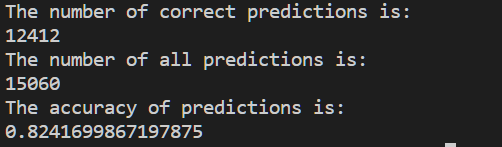
\includegraphics[width=15cm]{result.png}
\end{figure}
%\clearpage
%\bibliography{E:/Papers/LiuLab}
%\bibliographystyle{apalike}
\end{document}
%%% Local Variables:
%%% mode: latex
%%% TeX-master: t
%%% End:
